\documentclass[../../main.tex]{subfiles}
\begin{document}
\section{Definition und Beispiele kommutativer Ringe}

\begin{df}\label{3.1.1}
Ein \emph{kommutativer Ring}\index{kommutativer Ring@{\bf kommutativer Ring}} ist ein Tripel (d.h. 3-Tupel) $(A,+,\cdot)$, wobei $(A,+)$ eine abelsche Gruppe ist und $\cdot : A\times A\to A$ eine (meist unsichtbar oder infix geschriebene, d.h. man schreibt $ab$ oder $a\cdot b$ statt $\cdot(a,b)$) Abbildung mit folgenden Eigenschaften:
\begin{itemize}
\item[(\. K)] $\forall a,b\in A: ab = ba$\index{kommutativ@{\bf kommutativ}}
\item[(\. A)] $\forall a,b,c\in A: (ab)c=a(bc)$\index{assoziativ@{\bf assoziativ}}
\item[(\. N)] $\exists e\in A : \forall a\in A: ae=a$\index{neutrales Element@{\bf neutrales Element}}
\item[(D)] $\forall a,b,c\in A: a(b+c) = (ab)+(ac) \text{ "`distributiv"'}$\index{distributiv@{\bf distributiv}}
\end{itemize}
\end{df}

\begin{bem}\label{3.1.2}
\begin{enumerate}[\normalfont(a)]
\item Sind $e,e'\in A$ mit $\forall a\in A: ae =a = ae'$, so $e'=e'e\overset{\text{(\. K)}}=ee' = e$. Daher ist $e$ wie in (\. N) eindeutig bestimmt und man schreibt dafür $1$ statt $e$ (die "`Eins"' oder das "`Einselement"' des kommutativen Ringes).
\item Manchmal lässt man $\begin{Bmatrix}\text{(\. A)}\\\text{(\. N)}\end{Bmatrix}$ in der Definition \ref{3.1.1} weg und bezeichnet einen kommutativen Ring mit $\begin{Bmatrix}\text{(\. A)}\\\text{(\. N)}\end{Bmatrix}$ als $\begin{Bmatrix}\text{assoziativen}\\\text{unitären}\end{Bmatrix}$ kommutativen Ring. Statt "`unitärer Ring"' sagt man auch "`kommutativer Ring mit Eins"'.
\item Man nennt $\begin{Bmatrix}A\\(A,+)\end{Bmatrix}$ die \emph{zugrundeliegende}
$\begin{Bmatrix}\text{\emph{Menge}}\\\text{\emph{abelsche Gruppe}}\end{Bmatrix}$ oder die
$\begin{Bmatrix}\text{\emph{Trägermenge}}\index{kommutativer Ring@{\bf kommutativer Ring}!Trägermenge}\\\text{\emph{additive Gruppe}}\index{kommutativer Ring@{\bf kommutativer Ring}!additive Gruppe}\end{Bmatrix}$ und
$\begin{Bmatrix}+\text{ die Addition}\\\cdot\text{ die Multiplikation}\end{Bmatrix}$ von $(A,+,\cdot)$.
\item Wie bei abelschen Gruppen ist auch bei kommutativen Ringen ein unsauberer Sprachgebrauch üblich, z.B. "`Sei $A$ ein kommutativer Ring"' statt "`Sei $(A,+,\cdot)$ ein kommutativer Ring"' [$\to$ \ref{2.1.2} (e)].
\item Wegen (\. A) kann man beim Multiplizieren mehrerer Elemente eines kommutativen Ringes beliebig umklammern [$\to$ \ref{2.1.6}] und damit auf Klammern verzichten [$\to$ \ref{2.1.7}]. Weiter kann man die Elemente auch in beliebiger Reihenfolge multiplizieren [$\to$ \ref{2.1.9}].
\item Es gilt die Konvention "`Punkt vor Strich"', d.h. $\cdot$ bindet stärker als $+$ und $-$: ~$ab+cd$ steht für $(ab)+(cd)$
und $ab-cd$ steht für $(ab)-(cd)$.
\item (D) sagt nichts anderes, als dass für jedes $a\in A$ die Abbildung $A\to A, x\mapsto ax$ ein Gruppenendomorphismus von $(A,+)$ ist [$\to$ \ref{2.2.12}]. Insbesondere gilt $a\cdot 0 = 0$ für alle $a\in A$ und $a(-b)=-(ab)$ für alle $a,b\in A$ [$\to$ \ref{2.2.11}].
\end{enumerate}
\end{bem}

\begin{pro}\label{3.1.3}
Sei $A$ ein kommutativer Ring. Dann $\# A = 1 \iff 0=1$ in $A$.
\end{pro}
\begin{proof}
\begin{itemize}
\item["`$\Longrightarrow$"'] Ist $A=\left\{a\right\}$, so gilt $0=a=1$.
\item["`$\Longleftarrow$"'] Gelte $0_A = 1_A$. Dann gilt für jedes $a\in A$
\[a\overset{\text{(\. N)}}=a\cdot 1_A = a\cdot 0_A \overset{\text{\ref{3.1.2} (g)}}= 0_A,\]
also $A=\left\{0_A\right\}=\left\{1_A\right\}$.
\end{itemize}
\end{proof}

\begin{bsp}\mbox{}[$\to$ \ref{2.1.3}]\label{3.1.4}
\begin{enumerate}[\normalfont(a)]
\item $(\left\{a\right\},+,\cdot)$ mit $+,\cdot:\left\{a\right\}\times\left\{a\right\}\to \left\{a\right\}, (a,a)\mapsto a$ ist ein kommutativer Ring mit $0=a=1$.
\item $\Z,\Q,\R$ (mit gewöhnlicher Addition und Multiplikation) sind kommutative Ringe.
\item Sei $A$ eine Menge. Dann ist $(\Pow(A),+,\cdot)$ mit $+,\cdot:\Pow(A)\times \Pow(A)\to \Pow(A)$ definiert durch $B+C:=B\Delta C = (B\setminus C)\cup (C\setminus B)$ und $B\cdot C:=B\cap C$ für $B,C\in\Pow(A)$ ein kommutativer Ring. Es gilt $1=A$.
\item Genauso wie man in \ref{2.1.11} das direkte Produkt von abelschen Gruppen eingeführt hat, kann man auch das direkte Produkt von kommutativen Ringen über punktweise Addition und Multiplikation einführen (Übung).
Auf diese Weise ist insbesondere $A^{\N_0}$ ein kommutativer Ring. Man kann die abelsche Gruppe $A^{\N_0}$ aber auch mit einer anderen Multiplikation, der sogenannten \emph{Faltung}, zu einem kommutativen Ring machen. Da dies für uns wichtig sein wird, formulieren wir es in einem Satz.
\end{enumerate}
\end{bsp}

\begin{sat}\label{3.1.5}
Sei $A$ ein kommutativer Ring. Dann ist $(A^{\N_0},+,*)$ mit
\begin{align*}
f+g:\N_0&\to A, &&k\mapsto f(k)+g(k)&&\text{ und}\\
\underbrace{f*g}_\text{"`gefaltet"'}:\N_0&\to A, &&k\mapsto \sum_{i=0}^k f(i)\cdot g(k-i)&&\text{ für alle $f,g\in A^{\N_0}$}
\end{align*}
ein kommutativer Ring mit $1:\N_0\to A, 0\mapsto 1, k\mapsto 0$ für $k\in \N$.
\end{sat}
\begin{proof}
Wir wissen aus \ref{2.1.11} schon, dass $(A^{\N_0},+)$ eine abelsche Gruppe ist. Man rechnet nun als Übung (\. K), (\. A),(\. N) und (D) nach.
\end{proof}
\begin{center}
\begin{tikzpicture}
 \node(f0){$f(0)$};
 \node[below=0 of f0](f1){$f(1)$};
 \node[below=0 of f1](f2){$f(2)$};
 \node[below=0 of f2](f3){$\vdots$};
 \node[right=0 of f0](f0g0){$f(0)g(0)$};
 \node[right=0 of f0g0](f0g1){$f(0)g(1)$};
 \node[right=0 of f0g1](f0g2){$f(0)g(2)$}; 
 \node[right=0 of f0g2](f0g3){$\cdots$}; 
 \node[above=0 of f0g0](g0){$g(0)$};
 \node[above=0 of f0g1](g1){$g(1)$};
 \node[above=0 of f0g2](g2){$g(2)$};
 \node[above=0.2 of f0g3](g3){$\cdots$};
 \node[right=0 of f1](f1g0){$f(1)g(0)$};
 \node[right=0 of f1g0](f1g1){$f(1)g(1)$};
 \node[below=0.2 of f0g2](f1g2){$\cdots$}; 
 \node[below=.2 of f0g3](f1g3){$\cdots$}; 
 \node[right=0 of f2](f2g0){$f(2)g(0)$};
 \node[below=0.2 of f1g1](f2g1){$\cdots$};
 \node[below=0.2 of f1g2](f2g2){$\cdots$}; 
 \node[below=0.2 of f1g3](f2g3){$\cdots$};
 \node[below=0 of f2g0](f3g0){$\vdots$}; 
 \node[below=0 of f2g1](f3g1){$\vdots$};
 \node[below=0 of f2g2](f3g2){$\vdots$}; 
 \node[below=0 of f2g3](f3g3){$\vdots$};
 
 \draw (g2) -- (f2);
 \draw (g1) -- (f1);
 \draw (g3) -- (f3);
 
 \draw (-.5,0.4) -- (6.5,0.4);
 \draw (.5,1) -- (.5,-2.5);
\end{tikzpicture}\\
Faltung bildet Summen über die Diagonalen.
\end{center}

\begin{center}
(\. N):
\begin{tabular}{c|cccc}
 & 1 & 0 & 0 & $\cdots$\\\hline
 $f(0)$ & $f(0)$ & 0 & 0 & $\cdots$ \\
 $f(1)$ & $f(1)$ & 0 & 0 & $\cdots$ \\
 $f(2)$ & $f(2)$ & 0 & 0 & $\cdots$ \\
 $\vdots$ & $\vdots$ & $\vdots$ & $\vdots$ & $\cdots$
\end{tabular}
\qquad (\. A):
\begin{minipage}[h][][b]{0.5\textwidth}
\centering
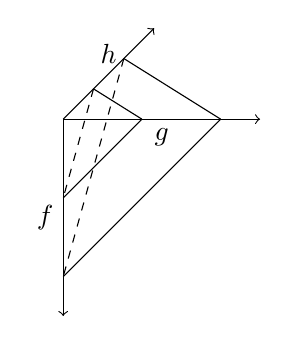
\begin{tikzpicture}
\draw[->] (0,0,0) -- node[above]{$h$} (0,0,-3);
\draw[->] (0,0,0) -- node[left]{$f$} (0,-2.5,0);
\draw[->] (0,0,0) -- node[below]{$g$} (2.5,0,0);

\draw[dashed] (0,0,-1) -- (0,-1,0);
\draw[dashed] (0,0,-2) -- (0,-2,0);

\draw (0,0,-1) -- (1,0,0);
\draw (0,0,-2) -- (2,0,0);

\draw (1,0,0) -- (0,-1,0);
\draw (2,0,0) -- (0,-2,0);
\end{tikzpicture}\\
Faltung bildet Summen über die Raumdiagonalen.
\end{minipage}
\end{center}

\begin{nt}\mbox{}[$\to$ \ref{2.1.10}]\label{3.1.6}
Sei $A$ ein kommutativer Ring [$\to$ \ref{3.1.1}]. Ist $(a_i)_{i\in I}$ eine Familie in $A$ und $n:=\# I\in\N$, so gilt $a_{\sigma(1)}\cdots a_{\sigma(n)} = a_{\tau(1)}\cdots a_{\tau(n)}$ für alle Bijektionen $\sigma,\tau:\left\{1,\ldots,n\right\}\to I$ [$\to$ \ref{2.1.6}, \ref{2.1.9}] und wir notieren dieses Element von $A$ mit $\prod_{i\in I} a_i$. Wir setzen $\prod_{i\in\emptyset} a_i := 1$. Statt $\prod_{i\in\left\{m,\ldots,n\right\}}a_i$ schreibt man auch $\prod_{i=m}^n a_i$. Beachte $\prod_{i=1}^0 a_i \overset{\text{\ref{1.1.6}}}=\prod_{i\in\emptyset}a_i = 1$. Für $n\in\N_0$ setzen wir weiter $a^n:=\prod_{i=1}^n a=\underbrace{a\cdots a}_\text{$n$-mal}$ (insbesondere $a^0=1$).
\end{nt}

\section{Unterringe, Ringhomomorphismen und Polynome}

\begin{df}\mbox{}[$\to$ \ref{2.2.1}]\label{3.2.1}
Seien $(A,+_A,\cdot_A)$ und $(B,+_B,\cdot_B)$ kommutative Ringe. Dann heißt $(B,+_B,\cdot_B)$ ein \emph{Unterring}\index{kommutativer Ring@{\bf kommutativer Ring}!Unterring} von $(A,+_A,\cdot_A)$, wenn $B\subseteq A,
\underline{\underline{1_A\in B}}, \forall a,b\in B: a+_B b = a+_A b$ und $\forall a,b\in B: a\cdot_B b = a\cdot_A b$.
\end{df}

\begin{pro}\label{3.2.2}{\rm[$\to$ \ref{2.2.2}]}
Sei $(A,+_A,\cdot_A)$ ein kommutativer Ring und $B$ eine Menge. Genau dann ist $B$ Trägermenge {\rm[$\to$ \ref{3.1.2} (c)]} eines Unterrings von $(A,+_A,\cdot_A)$, wenn $B$ Trägermenge einer Untergruppe von $(A,+_A)$ ist {\rm[$\to$ \ref{2.2.2}]} und $1_A\in B$ sowie $\forall a,b\in B: a\cdot_A b\in B$ gelten. In diesem Fall gibt es \emph{genau} ein Paar $(+_B,\cdot_B)$, mit dem $(B,+_B,\cdot_B)$ ein Unterring von $(A,+_A,\cdot_A)$ wird.\\
Es gilt dann $1_B=1_A, \forall a,b\in B:a\overset\cdot +_B b = a\overset\cdot +_A b$ und $\forall a\in B: -_Ba = -_A a$.
\end{pro}
\begin{proof}
Einfach mit \ref{2.2.2}.
\end{proof}

\red{Bis hierher sollten wir am 18. November kommen.}

\begin{bsp}\label{3.2.3}
\begin{enumerate}[\normalfont(a)]
\item $A:=\left\{0_\Z\right\}$ mit der gewöhnlichen Addition und Multiplikation ist ein kommutativer Ring (in dem $1_A=0_A=0_\Z$ gilt), aber kein Unterring von $\Z$, denn $1_\Z\notin A$.
\item Folgende Inklusionen sind Unterringbeziehungen: $\Z\subseteq \Q\subseteq\left\{a+b\sqrt{2}\mid a,b\in \Q\right\}\subseteq \R$ (beachte $(a+b\sqrt{2})(c+d\sqrt{2})=(ac+2bd)+(ab+bc)\sqrt{2}$ für alle $a,b,c,d\in \Q$).
\end{enumerate}
\end{bsp}

\begin{notsat}\label{3.2.4}
Sei $A$ ein kommutativer Ring, $B$ ein Unterring von $A$ und $x\in A$. Dann ist
$$\underbrace{B[x]}_\text{"`$B$ adjungiert $x$"'} :=\left\{\sum_{k=0}^n a_kx^k\mid n\in\N_0, a_0,\ldots,a_n\in B\right\}$$
der kleinste Unterring $C$ von $A$ mit $B\cup \left\{x\right\}\subseteq C$.
\end{notsat}
\begin{proof}
Zu zeigen:
\begin{enumerate}[\normalfont(a)]
\item $B[x]$ ist Unterring von $A$ mit $B\cup \left\{x\right\}\subseteq B[x]$.
\item Ist $C$ Unterring von $A$ mit $B\cup \left\{x\right\}\subseteq C$, so gilt $B[x]\subseteq C$.
\end{enumerate}
(b) ist klar.
Für (a) ist zu zeigen:
\begin{enumerate}[(1)]
\item $B\cup \left\{x\right\}\subseteq B[x]\subseteq A$
\item $\forall a,b\in B[x]:(a+b\in B[x]\et ab\in B[x])$
\item $\forall a\in B[x]:-a\in B[x]$
\end{enumerate}
\begin{enumerate}[Zu (1).]
\item Es gilt $a=a\cdot x^0\in B[x]$ für alle $a\in B$ und $x=1\cdot x^1\in B[x]$. Klar ist auch $B[x]\subseteq A$.
\item Seien $a,b\in B[x]$, etwa $a=\sum_{k=0}^m a_k x^k$ und $b=\sum_{k=0}^n b_k x^k$ mit\\ $m,n\in\N_0, a_0, \ldots, a_m,b_0, \ldots, b_n\in B$. Setze $a_k:=0$ für $k\geq m+1$ und $b_k:= 0$ für $k\geq n+1$. Dann gilt mit $\max\left\{m,n\right\}:=\text{größtes Element der Menge $\left\{m,n\right\}$}$:
$$a+b\overset{\text{\ref{2.1.9}}}=\sum_{k=0}^{\max\left\{m,n\right\}}(a_kx^k +b_kx^k)\overset{\text{(D)}}= \sum_{k=0}^{\max\left\{m,n\right\}}(\underbrace{a_k+b_k}_{\in B})x^k\in B[x] \text{ und}$$
$$ab\overset{\text{(D)}}=\sum_{k=0}^{m+n}\sum_{i=0}^{k}(a_ib_{k-i})x^k\in B[x]$$
\begin{center}
\begin{tikzpicture}
 \node(a0x0){$a_0x^0$};
 \node[below=0 of a0x0](a1x1){$a_1x^1$};
 \node[below=0 of a1x1](a2x2){$a_2x^2$};
 \node[below=0 of a2x2](a3x3){$\vdots$};
 \node[right=0 of a0x0](a0b0x0){$a_0b_0x^0$};
 \node[right=0 of a0b0x0](a0b1x1){$a_0b_1x^1$};
 \node[right=0 of a0b1x1](a0b2x2){$a_0b_2x^2$}; 
 \node[right=0 of a0b2x2](a0b3x3){$\cdots$}; 
 \node[above=0 of a0b0x0](b0x0){$b_0x^0$};
 \node[above=0 of a0b1x1](b1x1){$b_1x^1$};
 \node[above=0 of a0b2x2](b2x2){$b_2x^2$};
 \node[above=0.2 of a0b3x3](b3x3){$\cdots$};
 \node[right=0 of a1x1](a1b0x1){$a_1b_0x^1$};
 \node[right=0 of a1b0x1](a1b1x2){$a_1b_1x^2$};
 \node[below=0.2 of a0b2x2](a1b2x3){$\cdots$}; 
 \node[below=.3 of a0b3x3](a1b3x4){$\cdots$}; 
 \node[right=0 of a2x2](a2b0x2){$a_2b_0x^2$};
 \node[below=0.2 of a1b1x2](a2b1x3){$\cdots$};
 \node[below=0.2 of a1b2x3](a2b2x4){$\cdots$}; 
 \node[below=0.2 of a1b3x4](a2b3x5){$\cdots$};
 \node[below=0 of a2b0x2](a3b0x3){$\vdots$}; 
 \node[below=0 of a2b1x3](a3b1x4){$\vdots$};
 \node[below=0 of a2b2x4](a3b2x5){$\vdots$}; 
 \node[below=0 of a2b3x5](a3b3x6){$\vdots$};
 
 \node[right=0.2 of a0b3x3](a0b4x4){$0$};
 \node[right=0.2 of a1b3x4](a1b4x5){$0$};
 \node[right=0.2 of a2b3x5](a2b4x6){$0$};
 \node[below=0.2 of a2b4x6](a3b4x7){$0$};

 \node[below=0.1 of a3b0x3](a4b0x4){$0$};
 \node[below=0.1 of a3b1x4](a4b1x5){$0$};
 \node[below=0.1 of a3b2x5](a4b2x5){$0$};
 \node[below=0.1 of a3b3x6](a4b3x7){$0$};

 \node[right=0.4 of b3x3](dummy){};
 \node[below=0.1 of a3x3](dummy2){};

 \draw (b2x2) -- (a2x2);
 \draw (b1x1) -- (a1x1);
 \draw (b3x3) -- (a3x3);
 \draw (dummy) -- (dummy2);
 
 \draw (-.5,0.4) -- (6,0.4);
 \draw (-.5,-2.5) -- (5.5,-2.5);
 \draw (.5,1) -- (.5,-3);
 \draw (5.5,1) -- (5.5,-2.5);
\end{tikzpicture}
\end{center}
\item[(3)] ist klar.
\end{enumerate}
\end{proof}

\begin{bsp}\label{3.2.5}
$\Q[\sqrt{2}]=\left\{a+b\sqrt{2}\mid a,b\in\Q\right\}$, denn "`$\supseteq$"' ist klar und "`$\subseteq$"' gilt, da auf der rechten Seite ein Unterring von $\R$ steht [$\to$ \ref{3.2.3} (b)], der $\Q\cup \left\{\sqrt{2}\right\}$ enthält und $\Q[\sqrt{2}]$ der kleinste solche ist [$\to$ \ref{3.2.4}].
\end{bsp}

\begin{df}\label{3.2.6}
Sei $A$ ein kommutativer Ring. Ein kommutativer Ring $B$ heißt \emph{Polynomring}\index{kommutativer Ring@{\bf kommutativer Ring}!Polynomring} über $A$ in $x$, wenn $B=A[x]$ und 
$$\forall n\in\N_0:\forall a_0,\ldots,a_n \in A:\left(\sum_{k=0}^na_kx^k=0\Longrightarrow a_0=\ldots=a_n=0\right).$$
Man nennt dann die Elemente von $B$ \emph{Polynome}\index{Polynom@{\bf Polynom}} in
der \emph{Unbestimmten oder Variablen} $x$. Ist $p=\sum_{k=0}^n a_k x^k ~(a_k\in A)$ ein Polynom, so ist der \emph{$k$-te Koeffizient}\index{Polynom@{\bf Polynom}!Koeffizient} $a_k$ von $p$ eindeutig bestimmt (denn $\sum_{k} a_k x^k =\sum_k b_k x^k$ mit $a_k,b_k\in A$ impliziert $\sum_k(a_k-b_k)x^k=0$ und damit $a_k-b_k=0$ für alle $k$, d.h. $a_k=b_k$ für alle $k$).
Ist $p=\sum_{k=0}^n a_k x^k ~(a_k\in A)$ mit $a_n\neq 0$, so heißt $a_n$ der \emph{Leitkoeffizient}\index{Polynom@{\bf Polynom}!Koeffizient!Leitkoeffizient} oder \emph{höchste Koeffizient} von $p$ und $\underbrace{\deg}_\text{"`degree"'} p:= n$ der \emph{Grad} von $p$. Wir setzen $\deg(0) := -\infty$.
\end{df}

\begin{bsp}\label{3.2.7}
Ist $A=\left\{0\right\}$ ein einelementiger kommutativer Ring [$\to$ \ref{3.1.3}, \ref{3.1.4} (a)], so ist $A$ ein Polynomring über sich selber in $0$.
\end{bsp}

\begin{df}\mbox{}[$\to$ \ref{2.2.9}]\label{3.2.8}
Seien $(A,+_A,\cdot_A)$ und $(B,+_B,\cdot_B)$ kommutative Ringe. Dann heißt $f$ ein (Ring-)\emph{Homomorphismus}\index{kommutativer Ring@{\bf kommutativer Ring}!Homomorphismus} von $(A,+_A,\cdot_A)$ nach $(B,+_B,\cdot_B)$, wenn $f$ ein Gruppenhomomorphismus von $(A,+_A)$ nach $(B,+_B)$ ist mit $\underline{\underline{f(1_A)=1_B}}$ und $\forall a,b\in A: f(a\cdot_A b)=f(a)\cdot_B f(b)$.
\end{df}

\begin{bsp}\label{3.2.9}
\begin{enumerate}[\normalfont(a)]
\item $f:\R\to\R, x\mapsto 0$ ist kein Ringhomomorphismus, da $f(1)=0\neq 1$.
\item $f:\Q\to\R, x\mapsto x$ ist ein Ringhomomorphismus.
\item Sei $A$ eine Menge und $B\subseteq A$. Wie in \ref{3.1.4} (c) machen wir $\Pow(A)$ und $\Pow(B)$ zu einem kommutativen Ring vermöge der symmetrischen Mengendifferenz als Addition und dem Schnitt als Multiplikation. Dann ist $\Pow(A)\to \Pow(B), C\mapsto C\cap B$ ein Ringhomomorphismus (nachrechnen!).
\end{enumerate}
\end{bsp}

\begin{df}\mbox{}[$\to$ \ref{2.2.12}]\label{3.2.10}
Ein Ringhomomorphismus $f:A\to B$ heißt (Ring-) $\begin{Bmatrix}\text{\emph{Einbettung oder Mono-}}\\\text{\emph{Epi-}}\\\text{\emph{Iso-}}\end{Bmatrix}$\emph{morphismus}\index{kommutativer Ring@{\bf kommutativer Ring}!Homomorphismus!Monomorphismus}\index{kommutativer Ring@{\bf kommutativer Ring}!Homomorphismus!Epimorphismus}\index{kommutativer Ring@{\bf kommutativer Ring}!Homomorphismus!Isomorphismus}, wenn $f\begin{Bmatrix}\text{injektiv}\\\text{surjektiv}\\\text{bijektiv}\end{Bmatrix}$ ist. Einen Ringhomomorphismus $f:A\to A$ nennt man auch einen \emph{(Ring-)Endomorphismus}\index{kommutativer Ring@{\bf kommutativer Ring}!Homomorphismus!Endomorphismus} von $A$ und, falls er bijektiv ist, \emph{(Ring-)Automorphismus}\index{kommutativer Ring@{\bf kommutativer Ring}!Homomorphismus!Automorphismus} von $A$.
\end{df}

\begin{pro}{\rm[$\to$\ref{2.3.13}]}\label{imfsubring}
Seien $A$ und $B$ kommutative Ringe und $f\colon A\to B$ ein Ringhomomorphismus. Dann ist $\im f$ ein Unterring von $B$.
\end{pro}
\begin{proof}
Aus \ref{2.3.13} wissen wir schon, dass $\im f$ eine Untergruppe der additiven Gruppe von $B$ ist. Zu zeigen sind dann gemäß \ref{3.2.2} noch:
\begin{enumerate}[\normalfont(a)]
\item $1\in\im f$
\item $\forall a,b\in\im f:ab\in\im f$
\end{enumerate}
(a) folgt daraus, dass nach der Definition \ref{3.2.8} eines Ringhomomorphismus gilt $f(1)=1$. Um (b) zu zeigen, seien $a,b\in\im f$. Wähle dann $c,d\in A$ mit $f(c)=a$ und $f(d)=b$.
Es folgt $f(cd)\overset{\text{$f$ Hom.}}=f(c)f(d)=ab$ und damit $ab\in\im f$.
\end{proof}

\begin{sat}\label{polynomialringexists}
Sei $A$ ein kommutativer Ring mit $0\neq 1$ und $x\notin A$. Dann gibt es einen Polynomring über $A$ in $x$.
\end{sat}
\begin{proof}
Betrachte $(A^{\N_0},+,*)$ wie in \ref{3.1.5}. Es ist $\varphi:A\rightarrow A^{\N_0}, a\mapsto (a,0,0,0,\ldots)$ [$\to$ \ref{1.1.30} (c)] eine Ringeinbettung. Daher ist $\widehat{\varphi} :A\to \im \varphi$ ein Ringisomorphismus und
\[A':=\im\varphi=\left\{(a,0,0,0,\ldots)\mid a\in A\right\}\] ein Unterring von $A^{\N_0}$ gemäß \ref{imfsubring}. Da die Behauptung eine \emph{strukturelle} Aussage über $A$ macht (\ref{2.2.15} gilt sinngemäß natürlich auch für kommutative Ringe statt abelsche Gruppen), reicht es, die Behauptung für $A'$ statt $A$ zu zeigen, denn $A\cong A'$. Aus ähnlichen Gründen kann man nach Definition \ref{3.2.6} $x$ durch irgendein festes Element außerhalb von $A'$ austauschen. Wegen $0\neq 1$ gilt $(0,1,0,0,\ldots)\notin A'$ und wir können daher $x=(0,1,0,0,\ldots)$ annehmen. Wir behaupten, dass nun der Unterring $A'[x]$ [$\to$ \ref{3.2.4}] von $A^{\N_0}$ ein Polynomring über $A'$ in $x$ ist [$\to$ \ref{3.2.6}]. Seien hierzu $n\in\N_0$ und $a_0,\ldots,a_n\in A$ mit
\[\sum_{k=0}^n \underbrace{\widehat{\varphi} (a_k)x^k}_{\widehat{\varphi} (a_k)*x*\ldots*x}=0.\] Zu zeigen:
$\widehat{\varphi} (a_0)=\ldots=\widehat{\varphi} (a_n)=0$. Durch Induktion nach $k\in\N_0$ zeigt man
\[x^k=(\underbrace{0,0,\ldots,0}_{k\text{ Nullen}},1,0,0,\ldots).\] Daher $(a_0,\ldots,a_n,0,0,\ldots)=\sum_{k=0}^n\widehat{\varphi}(a_k)x^k=0=(0,0,0,\ldots)$. Also $a_0=\ldots=a_n=0$ und daher $\widehat{\varphi} (a_0)=\ldots=\widehat{\varphi} (a_n)=0$.
\end{proof}

\begin{bem}\label{writeax}
Schreibt man $A[X]$ mit großem $X$, so meint man meist stillschweigend, dass $A[X]$ ein Polynomring über $A$ in $X$ ist.
\end{bem}

\begin{sat}\label{substitution}
Seien $A$ und $B$ kommutative Ringe und $\varphi:A\to B$ ein Ringhomomorphismus. Sei $x\in B$. Dann gibt es genau einen Ringhomomorphismus $\psi:A[X]\to B$ mit $\psi|_A=\varphi$ und $\psi(X)=x$. Für jedes Polynom $p=\sum_k a_kX^k ~(a_k\in A)$ gilt $\psi(p)=\sum_k\varphi(a_k)x^k$. 
\end{sat}
\begin{proof}
Offensichtlich muss $\psi$ so definiert werden, wenn es ein Ringhomomorphismus mit $\psi|_A=\varphi$ und $\psi(X)=x$ sein soll. Dass man $\ps$ so definieren kann, liegt an der Eindeutigkeit der Koeffizienten eines Polynoms
[$\to$ \ref{3.2.6}]. Es bleibt für das so definierte $\psi$ zu zeigen:
\begin{enumerate}[\normalfont(a)]
\item $\psi|_A=\varphi$,
\item $\psi(X)=x$,
\item $\psi(1)=1$,
\item $\forall p,q\in A[X]:\psi(p+q)=\psi(p)+\psi(q)$,
\item $\forall p,q\in A[X]:\psi(pq)=\psi(p)\psi(q)$
\end{enumerate}
(a), (b), (c) sind klar nach Definition von $\psi$.\\
Für (d) und (e) seien $a_k,b_k\in A$ beliebig. 
\begin{itemize}
\item[Zu (d):] 
\begin{align*}
\psi\left(\sum_k a_kX^k+\sum_kb_kX^k\right)&\overset{\ref{2.1.10}}{\underset{\text{(D)}}=}\psi\left(\sum_k(a_k+b_k)X^k\right)\overset{\text{Def.}}{\underset{\text{von $\psi$}}=}\sum_k\varphi(a_k+b_k)x^k\\
&\overset{\varphi\text{ Hom.}}=\sum_k(\varphi(a_k)+\varphi(b_k))x^k \\
&\overset{\text{(D)}}{\underset{\ref{2.1.10}}=}\sum_k\varphi(a_k)x^k+\sum_k\varphi(b_k)x^k\\
&\overset{\text{Def.}}{\underset{\text{von $\psi$}}=}\psi\left(\sum_ka_kX^k\right)+\psi\left(\sum_kb_kX^k\right)
\end{align*}
\item[Zu (e):] 
\begin{align*}
\psi\left(\left(\sum_k a_k X^k\right)\left(\sum_k b_k X^k\right)\right)&\overset{\text{(D)}}=\psi\left(\sum_k\left(\sum_{i=0}^ka_ib_{k-i}\right)X^k\right)\\
&\overset{\text{Def.}}{\underset{\text{von $\psi$}}=}\sum_k\varphi\left(\sum_{i=0}^ka_ib_{k-i}\right)x^k\\
&\overset{\varphi\text{ Hom.}}=\sum_k\left(\sum_{i=0}^k\varphi(a_i)\varphi(b_{k-i})\right)x^k\\
&\overset{\text{(D)}}=\left(\sum_k\varphi(a_k)x^k\right)\left(\sum_k\varphi(b_k)x^k\right)
\end{align*}
\end{itemize}
\end{proof}

\begin{kor}\label{substitutioncor}
Sei $A$ ein Unterring des kommutativen Ringes $B$ und $x\in B$. Dann gibt es genau einen Ringhomomorphismus $\psi:A[X]\to B$ mit $\psi(a)=a$ für $a\in A$ und $\psi(X)=x$. Für jedes Polynom $p=\sum_ka_kX^k~(a_k\in A)$ gilt $\psi(p)=\sum_ka_kx^k$. Insbesondere gilt $\im\psi=A[x]$.
\end{kor}

\begin{nt}\label{writepx}
In der Situation von \ref{substitutioncor} schreibt man auch $p(x)$ ("`$p$ ausgewertet in $x$"') statt $\psi(p)$ (obwohl $p$ keine Funktion, sondern ein Polynom ist).
Da $\psi$ ein Ringhomomorphismus ist, gilt dann $(p+q)(x)=p(x)+q(x)$, $(pq)(x)=p(x)q(x)$ und $1(x)=1$ für $p,q\in A[X]$.\index{Polynom@{\bf Polynom}!p@$p(x)$}
\end{nt}

\begin{sat}\label{axisoay}
Seien $A[X]$ und $A[Y]$ Polynomringe über dem kommutativen Ring $A$ in $X$ bzw. $Y$. Dann gibt es genau einen Ringisomorphismus $\psi:A[X]\to A[Y]$ mit $\psi(a)=a$ für $a\in A$ und $\psi(X)=Y$.
\end{sat}
\begin{proof}
Nach \ref{substitutioncor} gibt es genau einen Ringhomomorphismus $\psi:A[X]\to A[Y]$ mit $\psi(a)=a$ für $a\in A$ und $\psi(X)=Y$. Offensichtlich gilt $\im \psi = A[Y]$, d.h. $\psi$ ist surjektiv. Noch zu zeigen: $\psi$ injektiv.

Es reicht $\ker\psi=\left\{0\right\}$ zu zeigen. Gelte hierzu $\psi\left(\sum_k a_k X^k\right)=0 ~(a_k\in A)$. Dann $\sum_k a_k Y^k=0$, also $a_k=0$ für alle $k$, da $A[Y]$ Polynomring über $A$ in $Y$. Daher $\sum_k a_kX^k=0$ wie gewünscht.
\end{proof}

\begin{spr}\label{thepolynomialring}
Wegen \ref{axisoay} spricht man oft auch von \emph{\underline{\underline{dem}}} Polynomring $A[X]$ über $A$ in $X$.
\end{spr}

\section[tocentry={Ideale und Quotientenringe}]{Ideale und Quotientenringe {\small [$\to$ §\ref{1.3},~§\ref{2.3}]}}\label{3.3}

\noindent
Idee: Grobe Sichtweise auf kommutative Ringe einnehmen.

\begin{df} \label{3.3.1}
Sei $A$ ein kommutativer Ring. Eine \emph{Kongruenzrelation}\index{Relation@{\bf Relation}!Kongruenzrelation ($\equiv$)} auf $A$ ist eine Kongruenzrelation $\equiv$ auf der additiven Gruppe von $A$
[$\to$\ref{2.3.1}], für die gilt:
\begin{equation}\tag{$*$}\label{star2}
\forall a,a',b,b'\in A:((a\equiv a' ~\et~ b\equiv b')\implies ab\equiv a'b')
\end{equation}
\end{df}

\begin{bem}\label{3.3.2}
In Definition \ref{3.3.1} drückt Bedingung \eqref{star2} gerade aus, dass
\begin{align*}
A/\mbox{$\equiv$}~\times~A/\mbox{$\equiv$}~&\to~A/\mbox{$\equiv$}\\
(\overline a,\overline b)&\mapsto\overline{ab}\quad(a,b\in A)
\end{align*}
wohldefiniert ist.
\end{bem}

\begin{satdef}\label{3.3.3}
Sei $A$ ein kommutativer Ring und $\equiv$ eine Kongruenzrelation auf $A$. Dann wird die Quotientengruppe $A/\mbox{$\equiv$}$ {\rm[$\to$\ref{2.3.3}]} vermöge der durch
$$\overline a\overline b:=\overline{ab}\qquad(a,b\in G)$$
festgelegten ("`vertreterweisen"') Multiplikation zu einem kommutativen Ring, den man den zu $\equiv$ gehörigen \emph{Quotientenring}\index{Relation@{\bf Relation}!Kongruenzrelation ($\equiv$)!Quotientenring} von $A$
nennt (auch "`$A$ nach $\equiv$"' oder "`$A$ modulo $\equiv$"'). In ihm gilt $1=\overline1$.
\end{satdef}

\begin{proof}
Aus \ref{2.3.3} wissen wir schon, dass $A$ bezüglich der Addition eine abelsche Gruppe bildet. Es sind daher nur noch (\.K), (\.A), (\.N) und (D) aus Definition \ref{3.1.1} nachzurechnen:
\begin{enumerate}
\item[(\.K)] $\overline a\,\overline b=\overline{ab}=\overline{ba}=\overline b\,\overline a$ für alle $a,b\in A$.
\item[(\.A)]  $(\overline a\,\overline b)\,\overline c=\overline{ab}\,\overline c=\overline{(ab)c}=\overline{a(bc)}=\overline a\,\overline{bc}=
\overline a\,(\overline b\,\overline c)$ für alle $a,b,c\in A$.
\item[(\.N)] Für $a\in A$ gilt $\overline a\,\overline1=\overline{a1}=\overline a$. Daher ist $1=\overline 1$.
\item[(D)] $\overline a\,(\overline b+\overline c)=\overline{a}\,\overline{b+c}=\overline{a(b+c)}=\overline{ab+ac}=\overline{ab}+\overline{ac}=\overline a\,\overline b+\overline a\,\overline c$ für alle $a,b,c\in A$.
\end{enumerate}
\end{proof}

\begin{df}\label{3.3.4}
Sei $A$ ein kommutativer Ring. Eine Untergruppe $I$ der additiven Gruppe von $A$ [$\to$\ref{3.1.2}(c)] heißt \emph{Ideal}\index{kommutativer Ring@{\bf kommutativer Ring}!Ideal} von $A$, wenn $\forall a\in A:\forall b\in I:ab\in I$.
\end{df}

\begin{pro}\label{3.3.5}
Sei $A$ ein kommutativer Ring und $I\subseteq A$. Genau dann ist $I$ ein Ideal von $A$, wenn folgende Bedingungen gelten:
\begin{enumerate}[\rm(a)]
\item $0\in I$
\item $\forall a,b\in I:a+b\in I$
\item $\forall a\in A:\forall b\in I:ab\in I$\label{aiit}
\end{enumerate}
\end{pro}
\begin{proof}
Dies folgt direkt aus \ref{2.2.2} und \ref{3.3.4}, denn wenn \eqref{aiit} gilt, so ist Bedingung \ref{2.2.2}(d) automatisch erfüllt, da dann
$$-a=-(a1)\overset{\text{\ref{3.1.2}(g)}}=a(-1)=(-1)a\overset{\text{(c)}}\in I$$
für alle $a\in I$.
\end{proof}

\begin{sat}\text{\rm[$\to$\ref{2.3.6}]} \label{3.3.6} Sei $A$ ein kommutativer Ring. Die Zuordnungen
\begin{align*}
\equiv&\mapsto\overline0\\
\equiv_I&\mapsfrom I
\end{align*}
vermitteln eine Bijektion zwischen der Menge der Kongruenzrelationen auf $A$ und der Menge der Ideale von $A$.
\end{sat}

\begin{proof}
Zu zeigen ist:
\begin{enumerate}[\normalfont(a)]
\item Ist $\equiv$ eine Kongruenzrelation auf $A$, so ist $\overline0$ ein Ideal von $A$.
\item Ist $I$ ein Ideal von $A$, so ist $\equiv_I$ eine Kongruenzrelation auf $A$.
\item Ist $\equiv$ eine Kongruenzrelation auf $A$, so $\equiv_{\overline0}~=~\equiv$.
\item Ist $I$ ein Ideal von $A$, so $\overset{-_I}0=I$.
\end{enumerate}
\medskip\noindent
{\bf Zu (a).} Sei $\equiv$ eine Kongruenzrelation auf $A$. Wir wissen aus \ref{2.3.4} (oder \ref{2.3.6}) schon, dass $\overline 0$ eine Untergruppe von $A$ ist. Gemäß Definition
\ref{3.3.4} bleibt $\forall a\in A:\forall b\in\overline0:ab\in\overline0$ zu zeigen. Seien hierzu $a\in A$ und $b\in\overline0$. Dann $a\equiv a$ und $b\equiv0$, woraus mit
\ref{3.3.1}$(*)$ folgt $$ab\equiv a0\overset{\text{\ref{3.1.2}(g)}}=0,$$das heißt $ab\in\overline0$.

\medskip\noindent
{\bf Zu (b).} Sei $I$ eine Ideal von $A$. Wir wissen aus \ref{2.3.6} schon, dass $\equiv_I$ ein Kongruenzrelation der additiven Gruppe von $A$ ist. Es bleibt \ref{3.3.1}$(*)$ zu zeigen. Seien
hierzu $a,a',b,b'\in A$ mit $a\equiv_Ia'$ und $b\equiv_Ib'$. Zu zeigen ist $ab\equiv_Ia'b'$. Nun gilt $b-b'\in I$ und daher auch $ab-ab'=a(b-b')\in I$. Genauso gilt $a-a'\in I$ und
damit auch $b'a-b'a'=b'(a-a')\in I$. Hiermit $ab\equiv_Iab'=b'a\equiv_Ib'a'=a'b'$ und daher $ab\equiv_Ia'b'$.

\medskip\noindent
{\bf (c) und (d)} folgen aus Satz \ref{2.3.6}.
\end{proof}

\begin{df}{\rm[$\to$\ref{2.3.7}]}\label{3.3.7}
Sei $I$ ein Ideal des kommutativen Ringes $A$. Dann nennt man $A/I:=A/\mbox{$\equiv_I$}$ den Quotientenring\index{Relation@{\bf Relation}!Kongruenzrelation ($\equiv$)!Quotientenring} (oder \emph{Restklassenring}) von $A$ nach (oder modulo) $I$.
Die Kongruenzklassen $\overset{-_I}{a~}$ ($a\in A$) {\rm[$\to$\ref{2.3.1}]} von $\equiv_I$ nennt man manchmal auch die \emph{Restklassen}\index{Relation@{\bf Relation}!Kongruenzrelation ($\equiv$)!Restklassen} von $I$ (in $A$).
\end{df}

\red{Bis hierher sollten wir am 22. November kommen.}

\begin{pro}{\rm[$\to$\ref{2.2.5}]}\label{3.3.8}
Sei $A$ ein kommutativer Ring und $M$ eine Menge von Idealen von $A$. Dann ist auch $\bigcap M$ ein Ideal von $A$ (mit $\bigcap\emptyset:=A$).
\end{pro}
\begin{proof}
Nach \ref{2.2.5} wissen wir schon, dass $\bigcap M$ eine Untergruppe der additiven Gruppe von $A$ ist. Nach Definition \ref{3.3.4} bleibt $\forall a\in A:\forall b\in\bigcap M:ab\in\bigcap M$ zu zeigen.
Seien hierzu $a\in A$ und $b\in\bigcap M$. Dann gilt für jedes $I\in M$, dass $b\in I$ und damit $ab\in I$, weil $I$ ein Ideal ist. Also gilt $ab\in\bigcap M$.
\end{proof}

\begin{satdef}{\rm[$\to$\ref{2.2.6}]}\label{3.3.9}
Sei $A$ ein kommutativer Ring und $E\subseteq A$. Dann gibt es \emph{\underline{das} kleinste} Ideal $I$ von $A$ mit $E\subseteq I$. Man nennt es das von $E$ in $A$ \emph{erzeugte Ideal}\index{kommutativer Ring@{\bf kommutativer Ring}!Ideal!erzeugtes Ideal} und notiert es mit $(E)_A$ oder (etwas unsauber) mit $(E)$.
\end{satdef}

\begin{proof}
Völlig analog zum Beweis von \ref{2.2.6} (benutze \ref{3.3.8} statt \ref{2.2.5}).
\end{proof}

\begin{sat}{\rm[$\to$\ref{2.2.7}]}\label{3.3.10}
Sei $A$ ein kommutativer Ring und $E\subseteq A$. Dann gilt
$$(E)_A=\left\{\sum_{i=1}^ma_ib_i\mid m\in\N_0,a_1,\dots,a_m\in A,b_1,\dots,b_m\in E\right\}.$$
\end{sat}
\begin{proof}
Der Beweis ist völlig analog zum Beweis von Satz \ref{2.2.7} und stellt gleichzeitig einen neuen Beweis für \ref{3.3.9} dar!
\end{proof}

\begin{df}\label{3.3.11}
Sei $A$ ein kommutativer Ring. Dann nennt man Ideale von $A$ der Form
$$(a_1,\dots,a_n):=(a_1,\dots,a_n)_A:=(\{a_1,\dots,a_n\})_A\overset{\text{(D)}}=\left\{\sum_{i=1}^nb_ia_i\mid b_1,\dots,b_n\in A\right\}$$
mit $n\in\N_0$ und $a_1,\dots,a_n\in A$ \emph{endlich erzeugt}\index{kommutativer Ring@{\bf kommutativer Ring}!Ideal!endlich erzeugt} (e.e.) und Ideale der Form
$$(a)=\{ba\mid b\in A\}$$ mit $a\in A$ \emph{Hauptideale}\index{kommutativer Ring@{\bf kommutativer Ring}!Ideal!Hauptideal} von $A$.
\end{df}

\begin{bsp}\label{3.3.12}
\begin{enumerate}[\normalfont(a)]
\item Für $n\in\Z$ gilt $(n)=\{bn\mid b\in\Z\}=\langle n\rangle$. Ist $n>0$, so gilt
$$\Z/(n)=\left\{\overset{-_{(n)}}{a~~~}\mid a\in\Z\right\}$$
und
 $\Z/(n)$ hat genau $n$ Elemente. Die additive Gruppe des Ringes $\Z/(n)$ ist die abelsche Gruppe $\Z/\langle n\rangle$.
 \item Betrachte $\Z/(9)$ und schreibe kurz $\overline a$ statt $\overset{-_{(9)}}{a~~~}=\overset{\equiv_{(9)}}{a~~~}$. Dann
 $\Z/(9)=\{\overline 0,\dots,\overline 8\}$, $\overline{10}=1$, $\overline{100}=\overline{10}~\overline{10}=\overline 1~\overline1=\overline1=1$,
 $\overline{1000}=1$ und so weiter. Es gilt $\overline{17368}=\overline1+\overline7+\overline3+\overline6+\overline8=\overline1+\overline8+\overline3+\overline6+\overline7=
 \overline9+\overline9+\overline7=\overline7$. Daher gilt $17368\equiv_{(9)}7$. Der Rest von $17368$ bei Division durch $9$ ist also $7$.
\end{enumerate}
\end{bsp}

\begin{sat}\label{3.3.13}
Jedes Ideal von $\Z$ ist ein Hauptideal von $\Z$.
\end{sat}

\begin{proof}
Sei $I$ ein Ideal von $\Z$. Ist $I=\{0\}$, so ist $I=(0)$. Also bleibt nur der Fall zu betrachten, dass es ein $n\in\N$ gibt mit $n\in I$. Wähle dann das kleinste solche $n$. Wir behaupten nun $I=(n)$. Die Inklusion $I\supseteq(n)$ ist klar. Um $I\subseteq(n)$ zu beweisen, sei $a\in I$. Zu zeigen ist $a\in(n)$. Da
$\Z/(n)=\left\{\overset{-_{(n)}}{0~~~},\dots,\overset{\text{---------}_{(n)}}{n-1~~~}\right\}$, gibt es $b\in\{0,\dots,n-1\}$ mit $a\equiv_{(n)}b$, das heißt $a-b\in(n)\subseteq I$. Wir wissen
$b\in I$ (denn $b\overset{a-b\in I}{\equiv_I}a\overset{a\in I}{\equiv_I}0$) und damit sogar $b=0$, da $n$ kleinstmöglich gewählt wurde. Es folgt $a\equiv_{(n)}b=0$ und daher
$a\in(n)$.
\end{proof}

\begin{kor}\label{3.3.14}
Sei $H$ eine Untergruppe von $\Z$. Dann gilt $H=\langle n\rangle$ für ein $n\in\Z$.
\end{kor}

\begin{proof}
Jede Untergruppe der abelschen Gruppe $(\Z,+)$ ist ein Ideal des kommutativen Ringes $(\Z,+,\cdot)$, denn Multiplizieren mit einer ganzen Zahl lässt sich durch iteriertes
Addieren oder Subtrahieren ausdrücken.
\end{proof}

\begin{defprop}\label{3.3.15}[$\to$\ref{2.3.10}]
Seien $A$ und $B$ kommutative Ringe und $f\colon A\to B$ ein Homomorphismus. Dann ist $\equiv_f~$ eine Kongruenzrelation auf $A$ und
$\ker f$ ein Ideal von $A$.
\end{defprop}

\begin{proof}
Da sich $\equiv_f~$ und $\ker f$ nach \ref{2.3.10} unter der Bijektion aus Satz \ref{3.3.6} entsprechen, reicht es eine der beiden Behauptungen zu zeigen. Wir entscheiden uns für die
zweite. Dass $\ker f$ eine Untergruppe der additiven Gruppe von $A$ ist, wurde schon in \ref{2.3.10}(b) gezeigt. Nach Definition \ref{3.3.4} reicht es daher
$\forall a\in A:\forall b\in\ker f:ab\in\ker f$ zu zeigen. Sind nun $a\in A$ und $b\in\ker f$, so gilt $f(b)=0$ und daher $$f(ab)=f(a)f(b)=f(a)~0\overset{\ref{3.1.2}(g)}=0,$$
also $ab\in\ker f$.
\end{proof}

\begin{sat}[Homomorphiesatz für kommutative Ringe]\label{3.3.16}{\rm[$\to$\ref{2.3.11}]}
Seien $A$ und $B$ kommutative Ringe, $I$ ein Ideal von $A$ und $f\colon A\to B$ ein Homomorphismus
mit $I\subseteq\ker f$.
\begin{enumerate}[\rm(a)]
\item
Es gibt genau eine Abbildung $\overline f\colon A/I\to B$ mit
$\overline f(\overset{-_I}a)=f(a)$ für alle $a\in A$. Diese Abbildung $\overline f$ ist ein Homomorphismus.
\item
$\text{$\overline f$ ist injektiv}\iff I=\ker f$
\item
$\text{$\overline f$ ist surjektiv}\iff\text{$f$ ist surjektiv.}$
\end{enumerate}
\end{sat}
\begin{proof}
Existenz und Eindeutigkeit der Abbildung $\overline f$ erhält man dem Homomorphiesatz für abelsche Gruppen \ref{2.3.11}.
Dass $\overline f$ ein Gruppenhomomorphismus ist, wissen wir ebenfalls aus \ref{2.3.11}. Wir rechnen nach, dass $\overline f$ ein Ringhomomorphismus [$\to$\ref{3.2.8}] ist, wobei
wir $\equiv~:=~\equiv_I$ und damit $\overline a=\overset{-_I}a=\overset{\equiv_I}a$ für alle $a\in A$ schreiben:
$$\overline f(1)\overset{\text{\ref{3.3.3}}}=\overline f(\overline 1)\overset{\text{Def. von $\overline f$}}=f(1)\overset{\text{$f$ Hom.}}{\underset{\ref{3.2.8}}=}1\qquad\text{und}$$
und
$$\overline f(\overline a\,\overline b)\overset{\text{\ref{3.3.3}}}=\overline f(\overline{ab})\overset{\text{Def. von $\overline f$}}=f(ab)\overset{\text{$f$ Hom.}}{\underset{\ref{3.2.8}}=}f(a)f(b)
\overset{\text{Def. von $\overline f$}}=\overline f(\overline a)\,\overline f(\overline b)
$$
für alle $a,b\in A$.
Teil (b) und (c) der Behauptung folgen unmittelbar aus \ref{2.3.11}.
\end{proof}

\begin{bem}{\rm[$\to$\ref{2.3.12}]}\label{3.3.17}
Sei $I$ ein Ideal des kommutativen Ringes $A$. Dann wird $I$ durch einen Ringhomomorphismus
$f\colon A\to B$ in einen weiteren kommutativen Ring $B$ induziert, nämlich durch den \emph{kanonischen Epimorphismus}
$$f\colon A\to A/I,\ a\mapsto\overset{-_I}a.$$
In der Tat gilt $\ker f=I$ nach \ref{2.3.12}.
\end{bem}

\begin{kor}[Isomorphiesatz für kommutative Ringe]\label{isothmring} {\rm[$\to$\ref{2.3.14}]}
Seien $A$ und $B$ kommutative Ringe und $f\colon A\to B$ ein Homomorphismus.
Dann ist $\overline f\colon A/\ker f\to\im f$
definiert durch $\overline f(\overset{-_{\ker f}}{a~~})=f(a)$ für $a\in A$ ein Isomorphismus {\rm[$\to$\ref{3.2.10}]}. Insbesondere $A/\ker f\cong\im f$ (in der zu \ref{2.2.15} analogen Bedeutung).
\end{kor}
\end{document}